\subsubsection{MF4. Módulo de interfaz de usuario}

La interfaz de usuario de nuestra aplicación cuenta con un estilo de diseño neumorfista, respondiendo a las tendencias de diseño actuales, lo que genera una seguridad de uso 
para una aplicación moderna de carácter profesional, con una estética atractiva, consistencia visual, pero sobre todo interactividad y enfoque en el funcionamiento, permitiendo 
a los usuarios interactuar con el sistema de manera eficiente. A continuación, se describe el flujo de trabajo de la interfaz de usuario \ref{fig:diagrama_flujo}. \\

\begin{figure}[!htb]
    \centering
    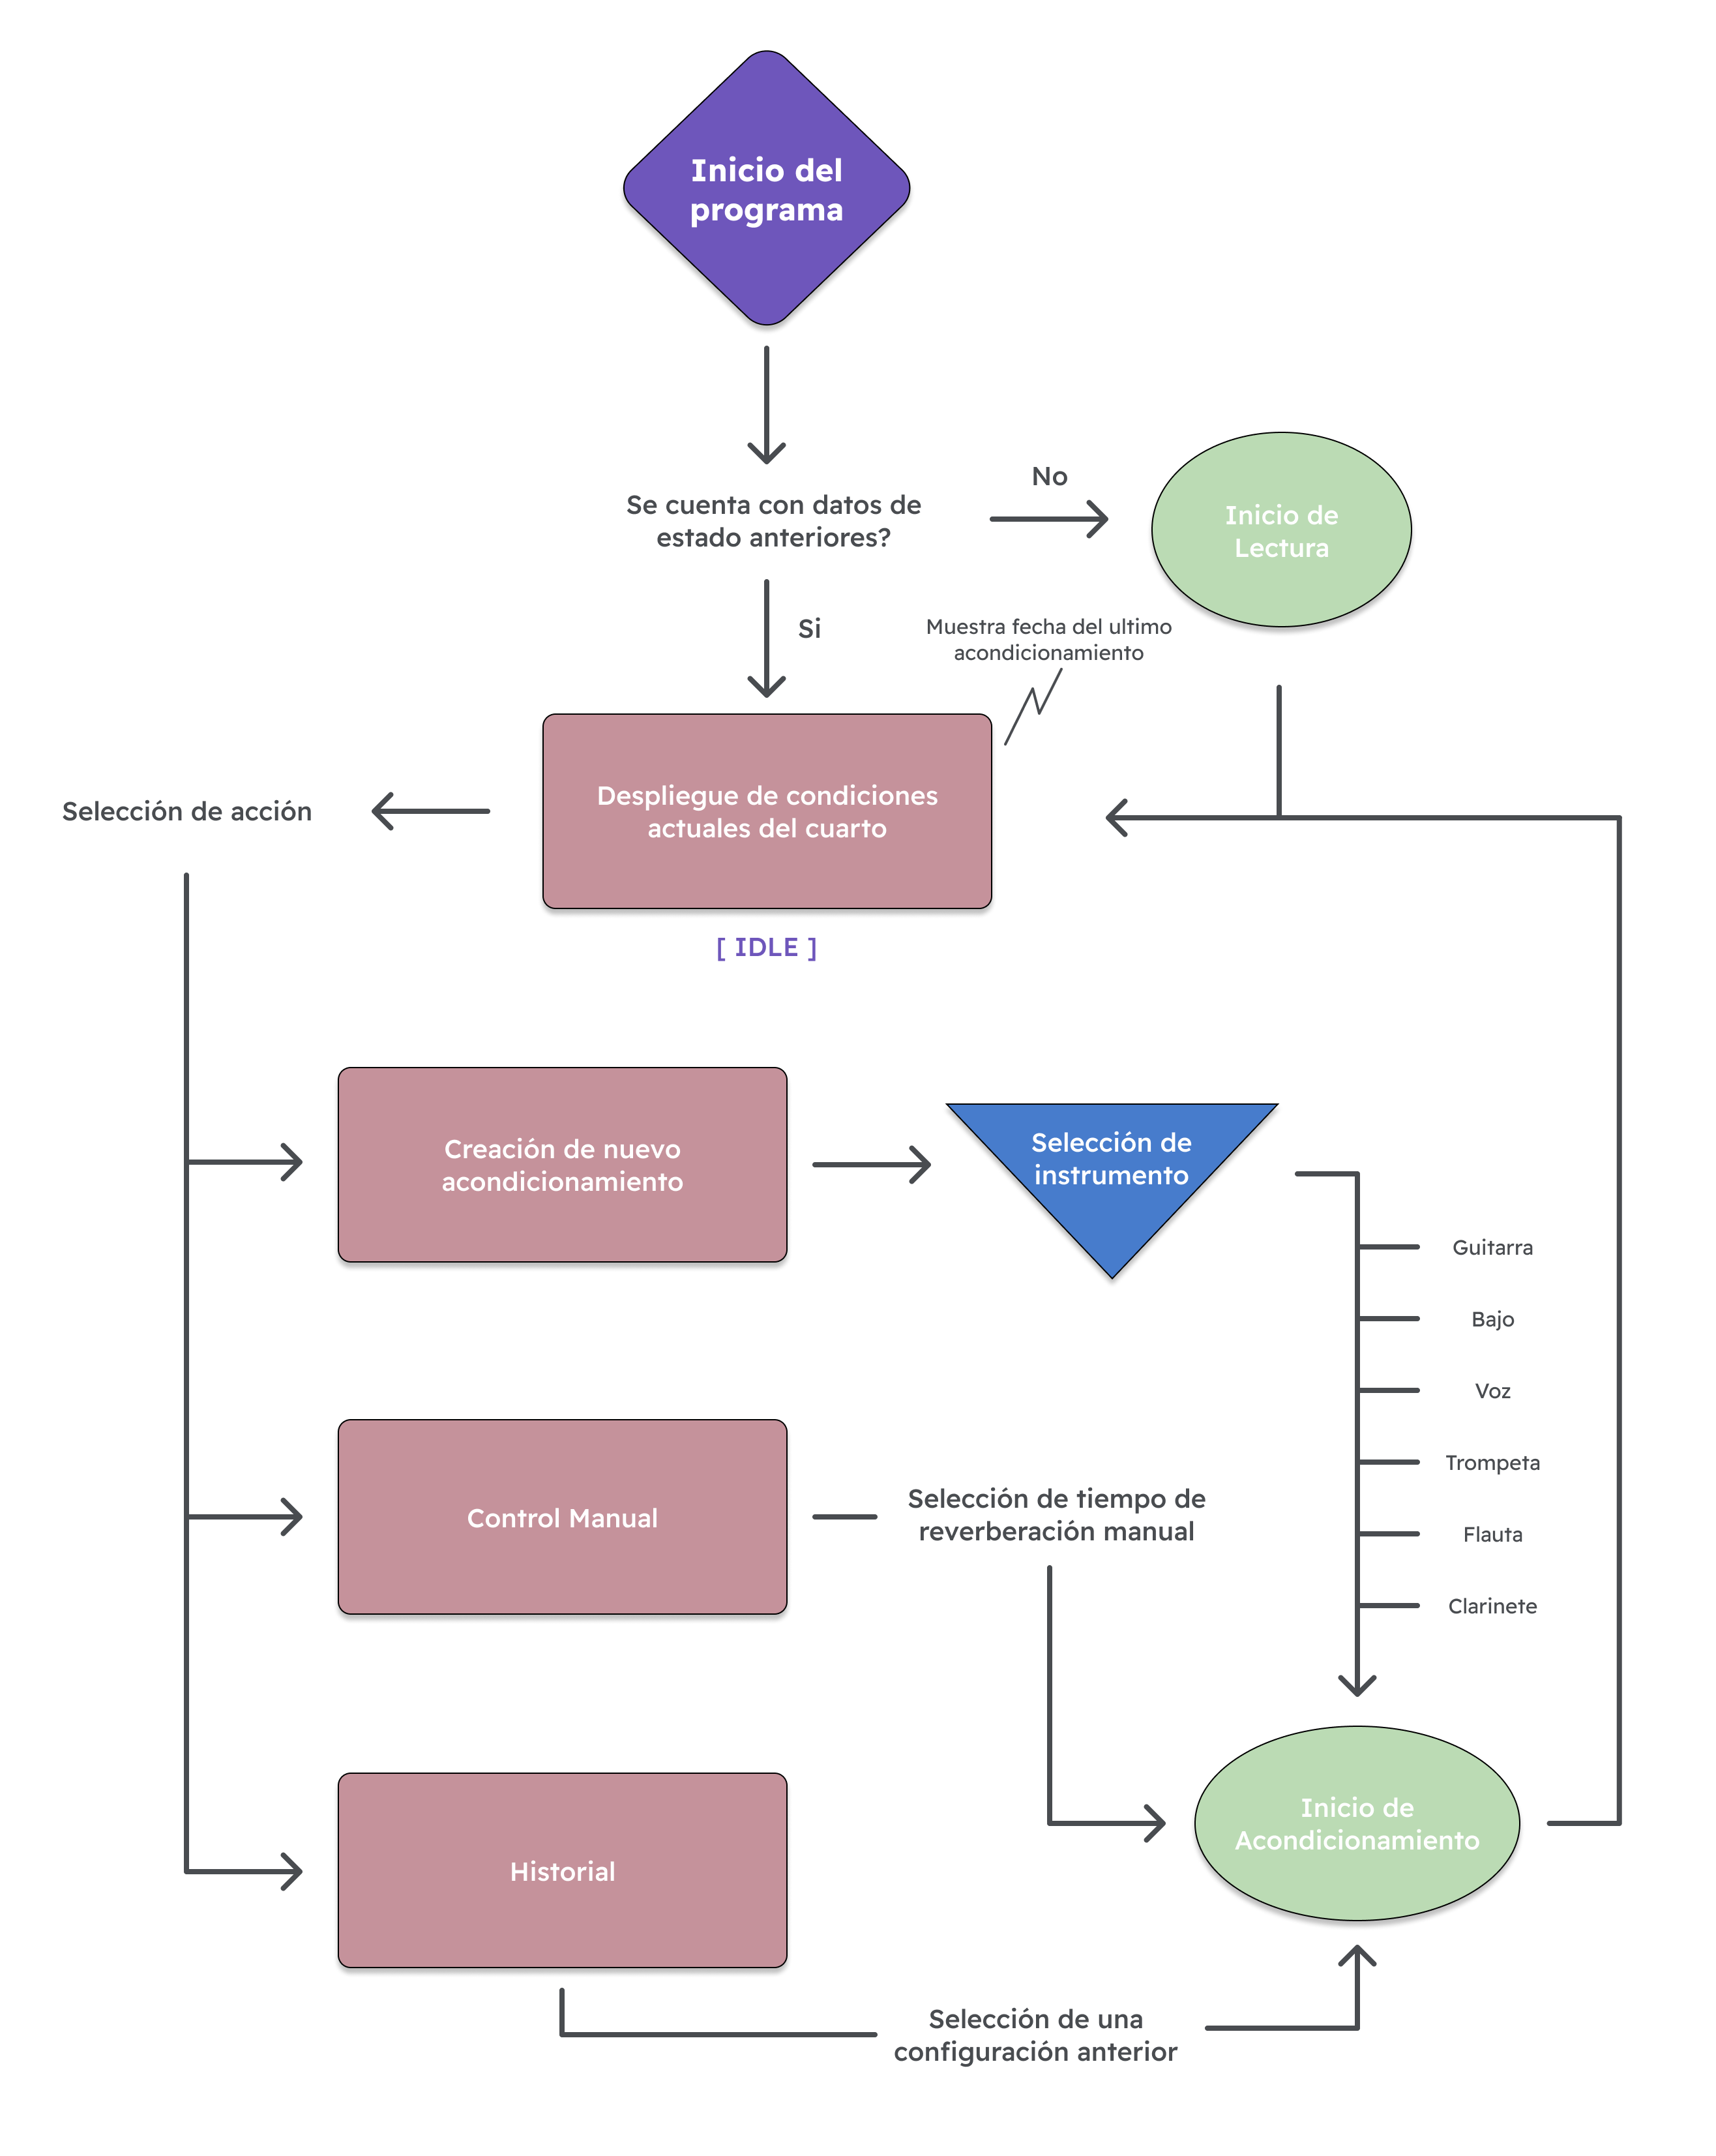
\includegraphics[width=1\linewidth]{imagenes/Diagrama de Flujo.png}
    \caption{Diagrama de Flujo de la aplicación}
    \label{fig:diagrama_flujo}
\end{figure}

Al iniciar el programa, el sistema verifica si hay datos de estado anteriores disponibles para mostrar: \\

\begin{itemize}[label={}, leftmargin=0pt]
    \item \textbf{Inicio del Programa:} El sistema comienza verificando si existen datos de estado previos.
    \item \textbf{Datos de Estado Anteriores:}
    \begin{itemize}
        \item \textbf{Sí:} Si hay datos de estado anteriores, se despliegan las condiciones actuales del cuarto, incluyendo la fecha del último acondicionamiento (MF4.1.).
        \item \textbf{No:} Si no hay datos de estado previos, se inicia el proceso de lectura de datos actuales (MF4.2.). \\
    \end{itemize}
\end{itemize}

Una vez desplegadas las condiciones actuales del cuarto, el sistema se encuentra en estado de reposo, el usuario puede elegir entre las acciones: \\

\begin{itemize}[label={}, leftmargin=0pt]
    \item \textbf{Creación de Nuevo Acondicionamiento:} 
    \begin{itemize}
        \item El usuario selecciona esta opción para iniciar un nuevo acondicionamiento.
        \item \textbf{Selección de Instrumento:} El usuario elige el tipo de instrumento (Guitarra, Bajo, Voz, Trompeta, Flauta, Clarinete).
        \item \textbf{Inicio de Acondicionamiento:} Una vez seleccionado el instrumento, se inicia el acondicionamiento del cuarto.
    \end{itemize}
    \item \textbf{Control Manual:}
    \begin{itemize}
        \item El usuario puede ajustar manualmente el tiempo de reverberación.
        \item \textbf{Inicio de Acondicionamiento:} Después de ajustar manualmente, se procede con el acondicionamiento.
    \end{itemize}
    \item \textbf{Historial:}
    \begin{itemize}
        \item El usuario puede revisar el historial de acondicionamientos previos.
        \item \textbf{Selección de Configuración Anterior:} El usuario puede seleccionar una configuración anterior para replicarla.
        \item \textbf{Inicio de Acondicionamiento:} Una vez seleccionada, se inicia el acondicionamiento. \\
    \end{itemize}
\end{itemize}

La interfaz está compuesta por elementos que facilitan la interacción del usuario con el sistema, estos son: \\

\begin{itemize}[label={}, leftmargin=0pt]
    \item \textbf{Panel de Navegación:} Situado en el lado izquierdo de la pantalla, este panel permite al usuario navegar entre las diferentes secciones de la aplicación, como la visualización de condiciones actuales, la creación de nuevos acondicionamientos, el control manual y el historial.
    \item \textbf{Botón de Iniciar Lectura:} Este botón permite al usuario iniciar la lectura de las condiciones actuales del cuarto en cualquier momento.
    \item \textbf{Estado de Conexión:} Un indicador de conexión muestra si el sistema está conectado correctamente o si ha ocurrido algún fallo.
    \item \textbf{Principal:} Donde se encuentra la información de la diferentes acciones accesibles por el panel de navegación. Es la sección principal de la interfaz y varia su contenido según la pagina en la que se esté ubicado.
\end{itemize}

Finalmente podemos observar las imágenes en la Figura \ref{fig:vistas_interfaz} de las diferentes vistas de la interfaz. \\

\begin{figure}[!htb]
    \centering
    \begin{subfigure}{0.45\textwidth}
        \centering
        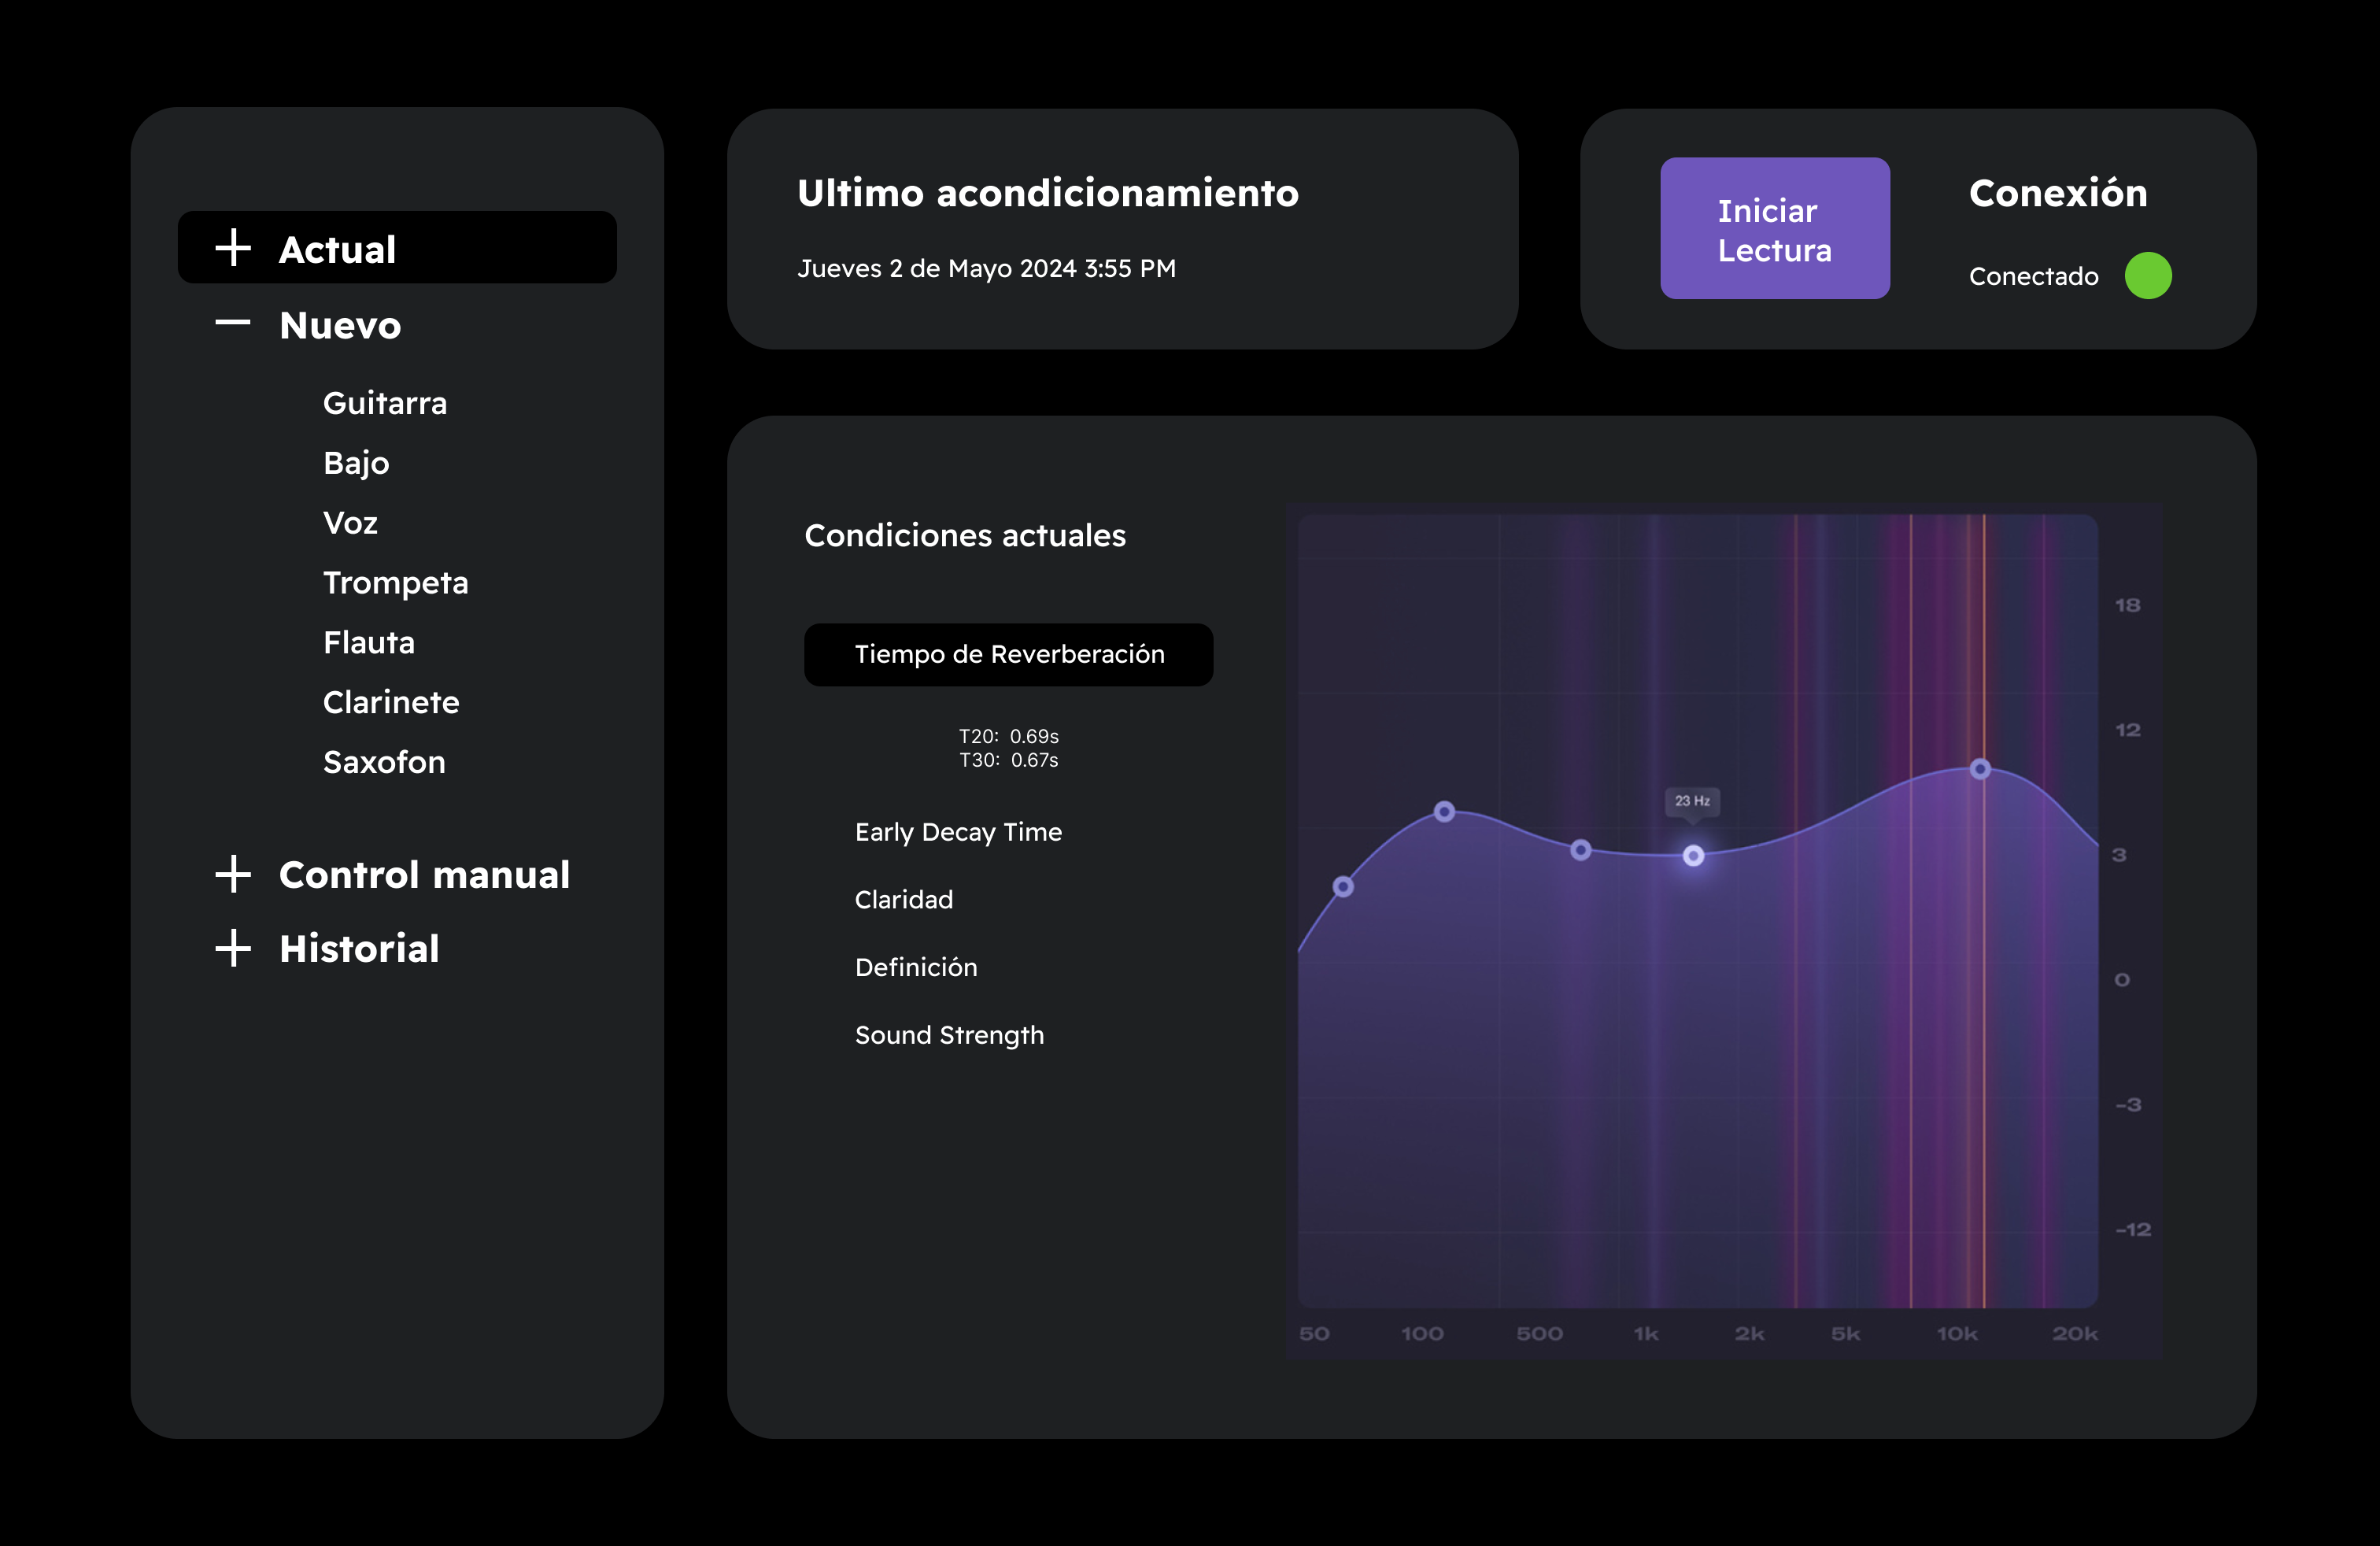
\includegraphics[width=\linewidth]{imagenes/Landing.png}
        \caption{\footnotesize Página de la acústica actual}
        \label{fig:pagina_home}
    \end{subfigure}
    \hfill
    \begin{subfigure}{0.45\textwidth}
        \centering
        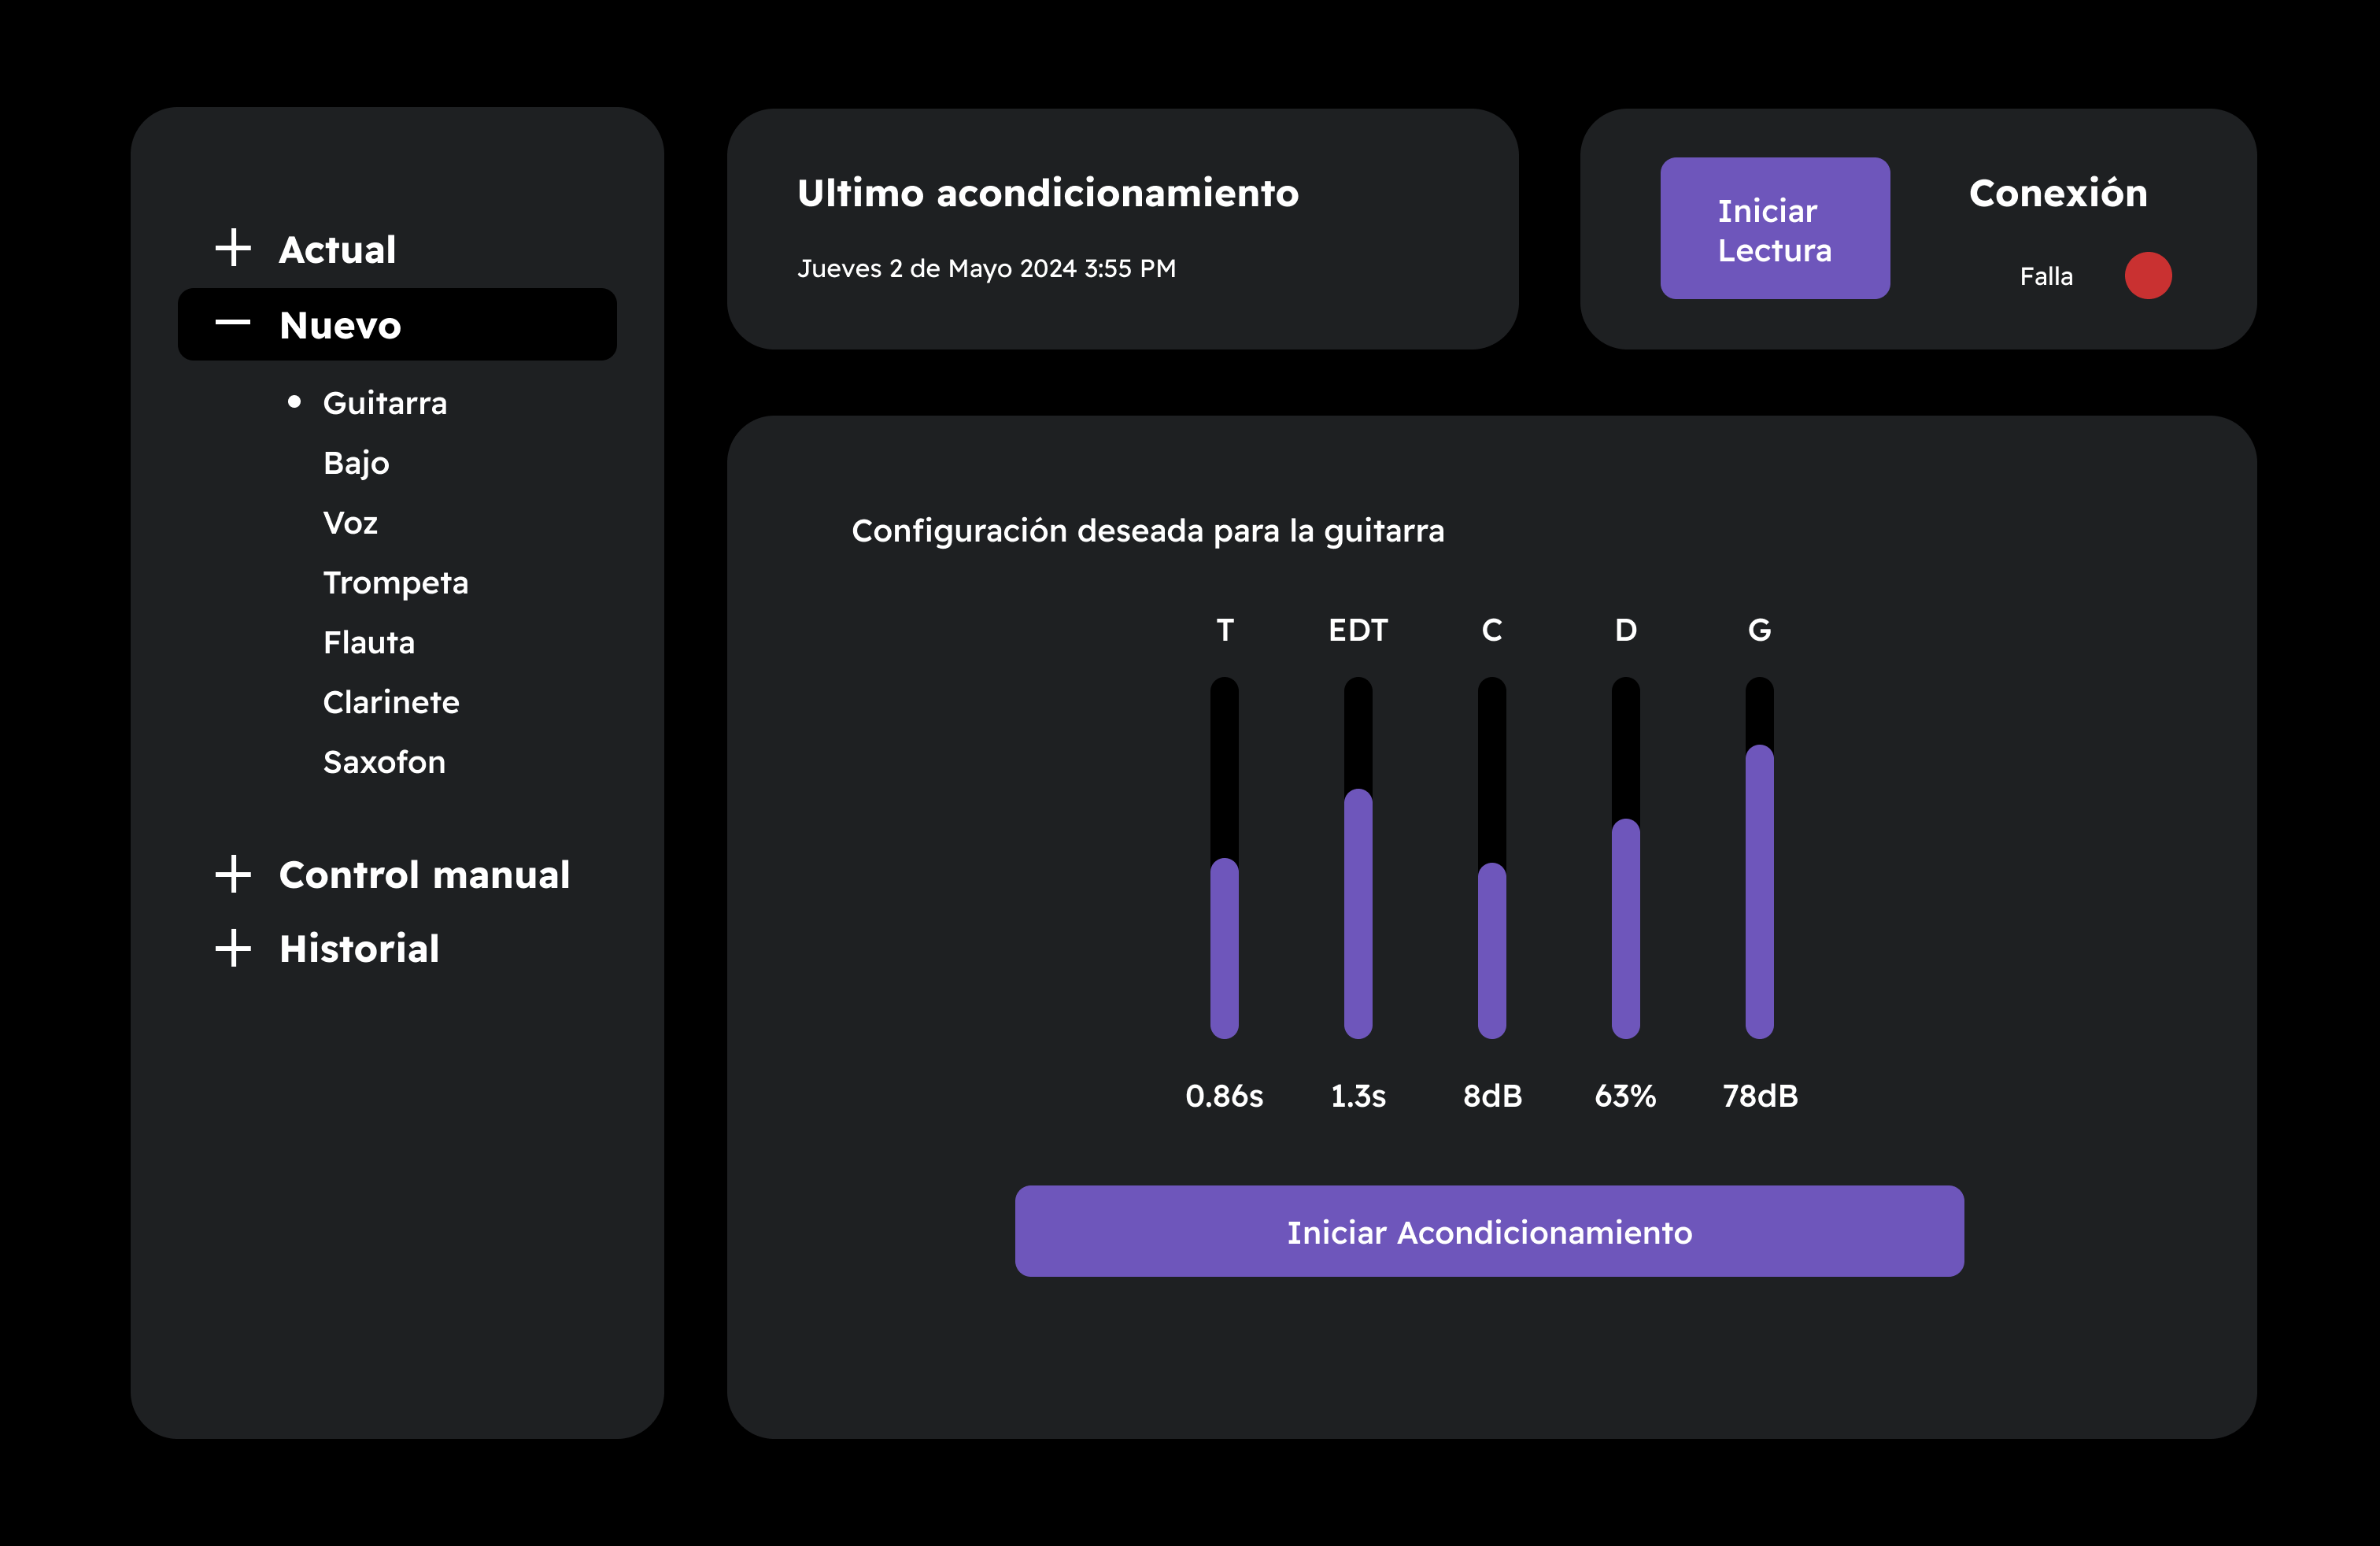
\includegraphics[width=\linewidth]{imagenes/Guitarra.png}
        \caption{\footnotesize Página generación de una nueva acústica}
        \label{fig:pagina_instrumento}
    \end{subfigure}
    \vskip\baselineskip
    \begin{subfigure}{0.45\textwidth}
        \centering
        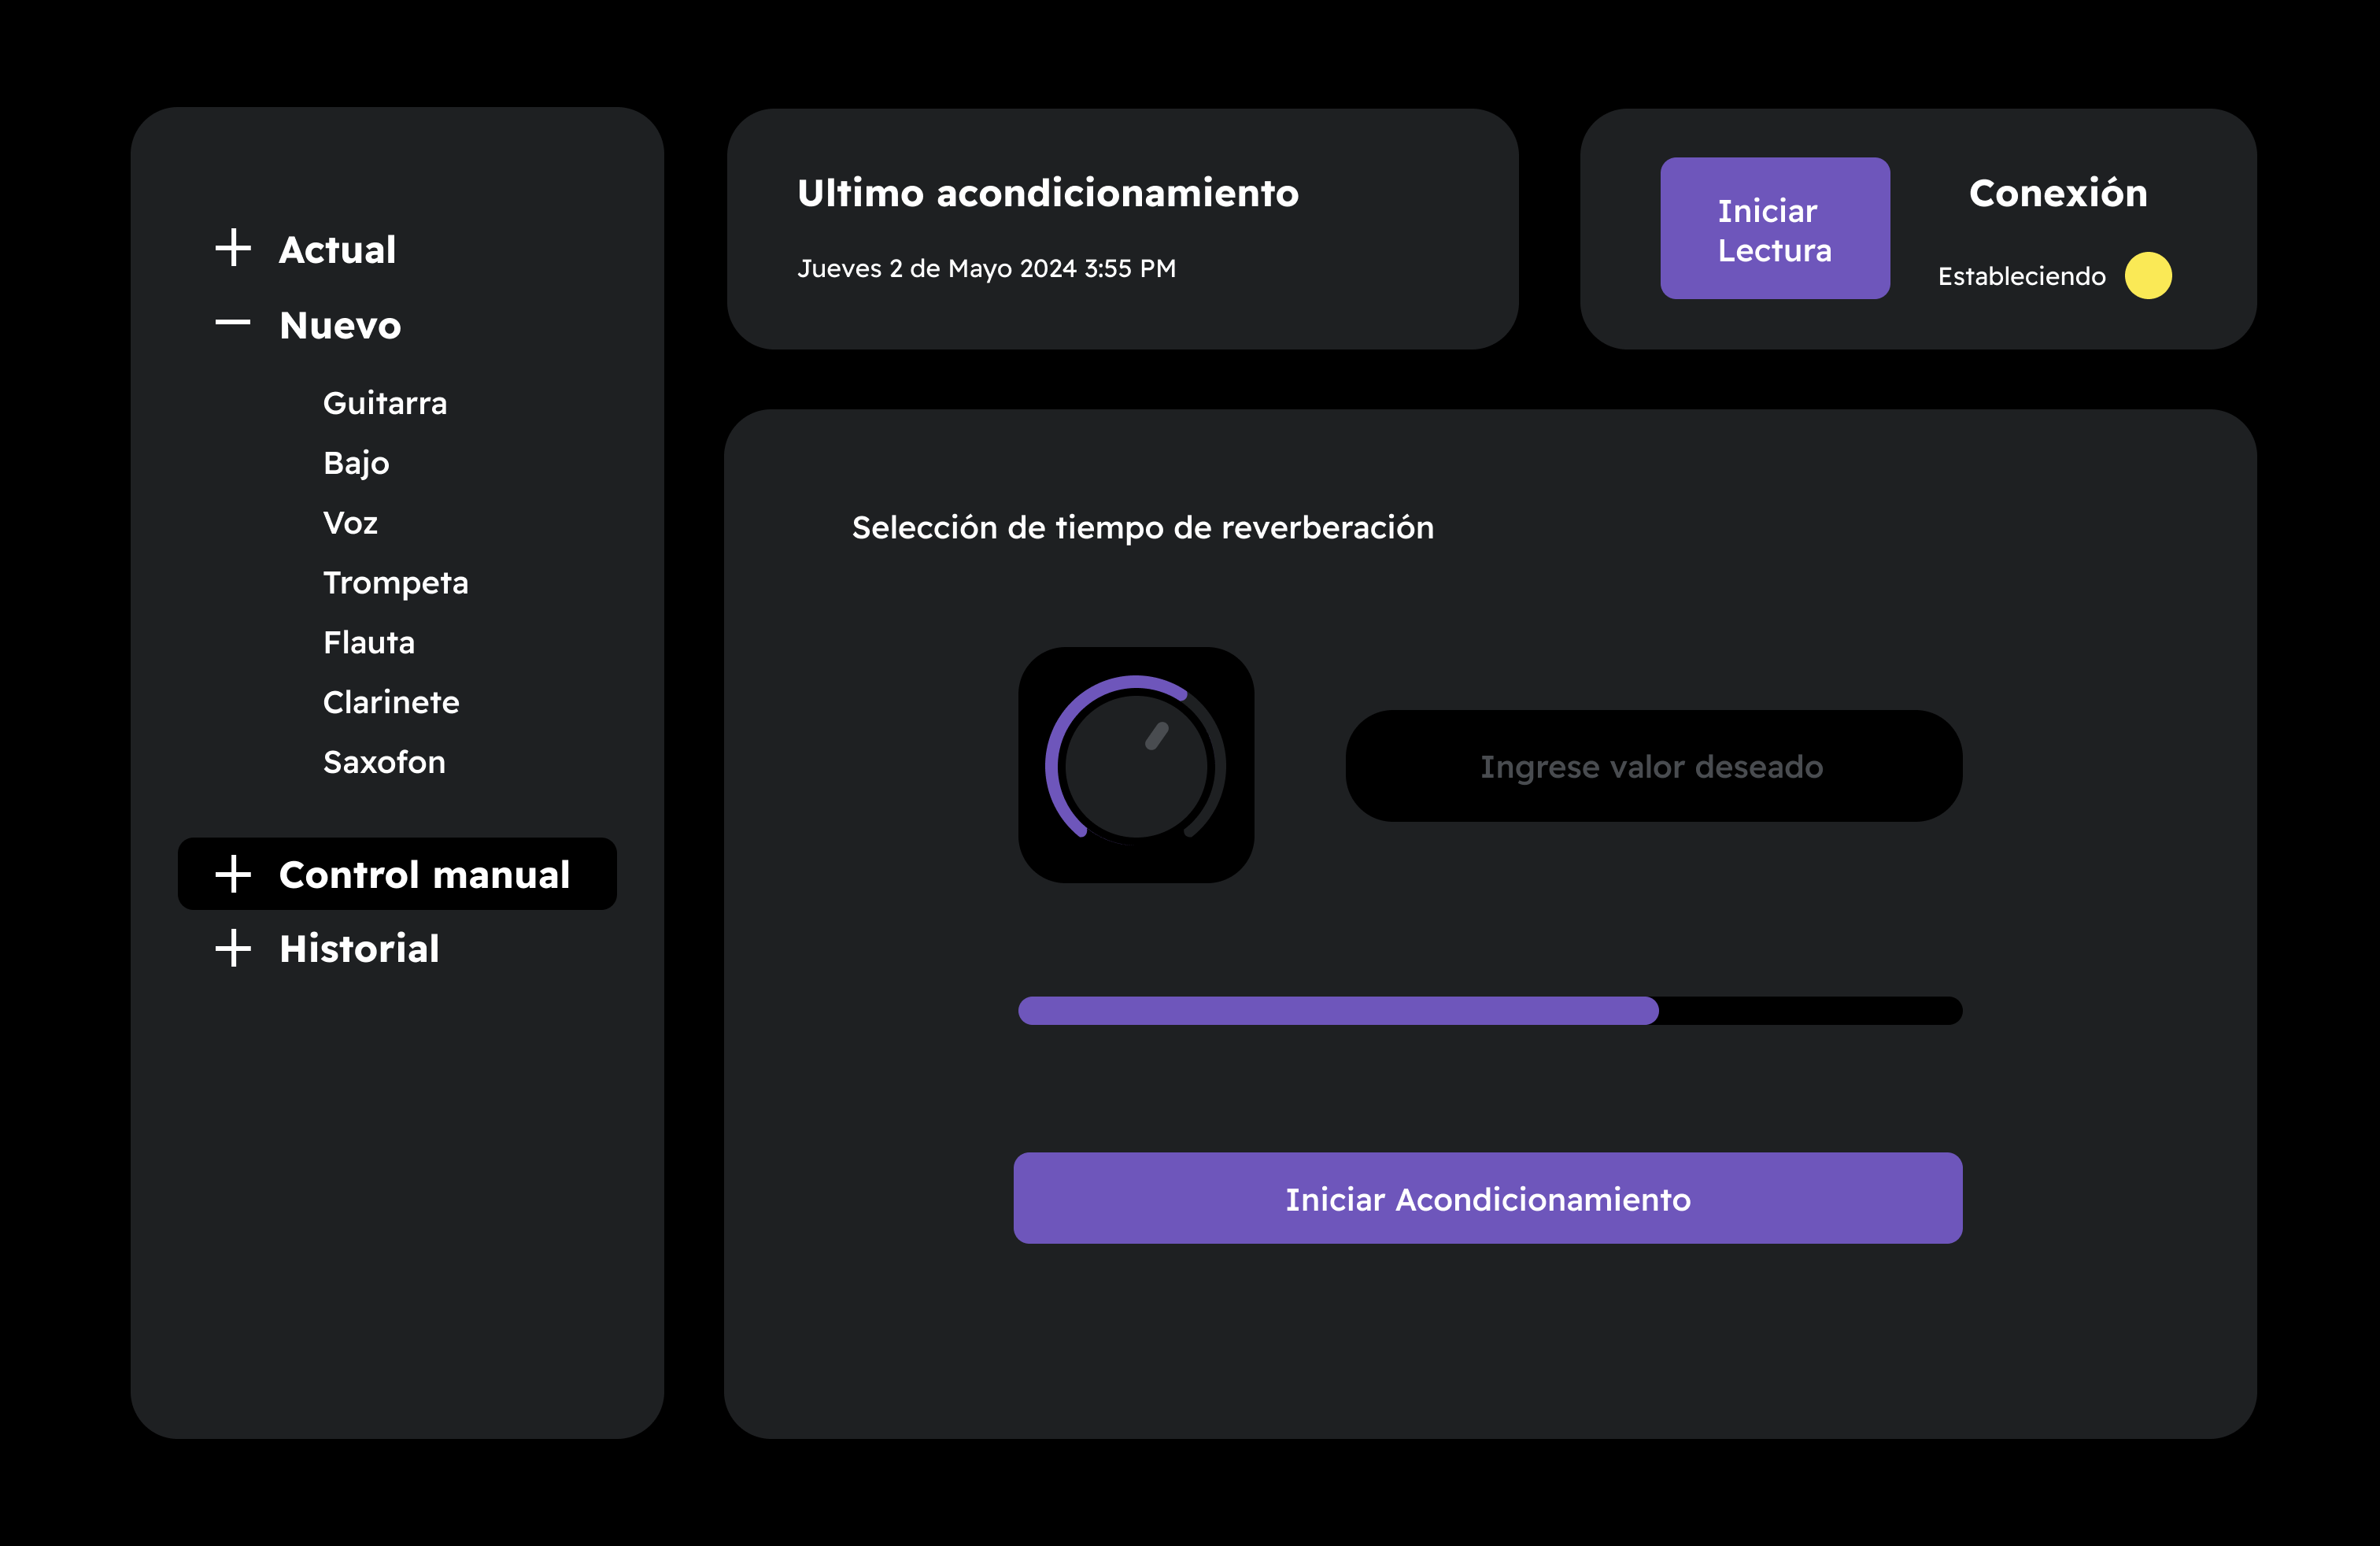
\includegraphics[width=\linewidth]{imagenes/Control Manual.png}
        \caption{\footnotesize Página de control manual}
        \label{fig:pagina_manual}
    \end{subfigure}
    \hfill
    \begin{subfigure}{0.45\textwidth}
        \centering
        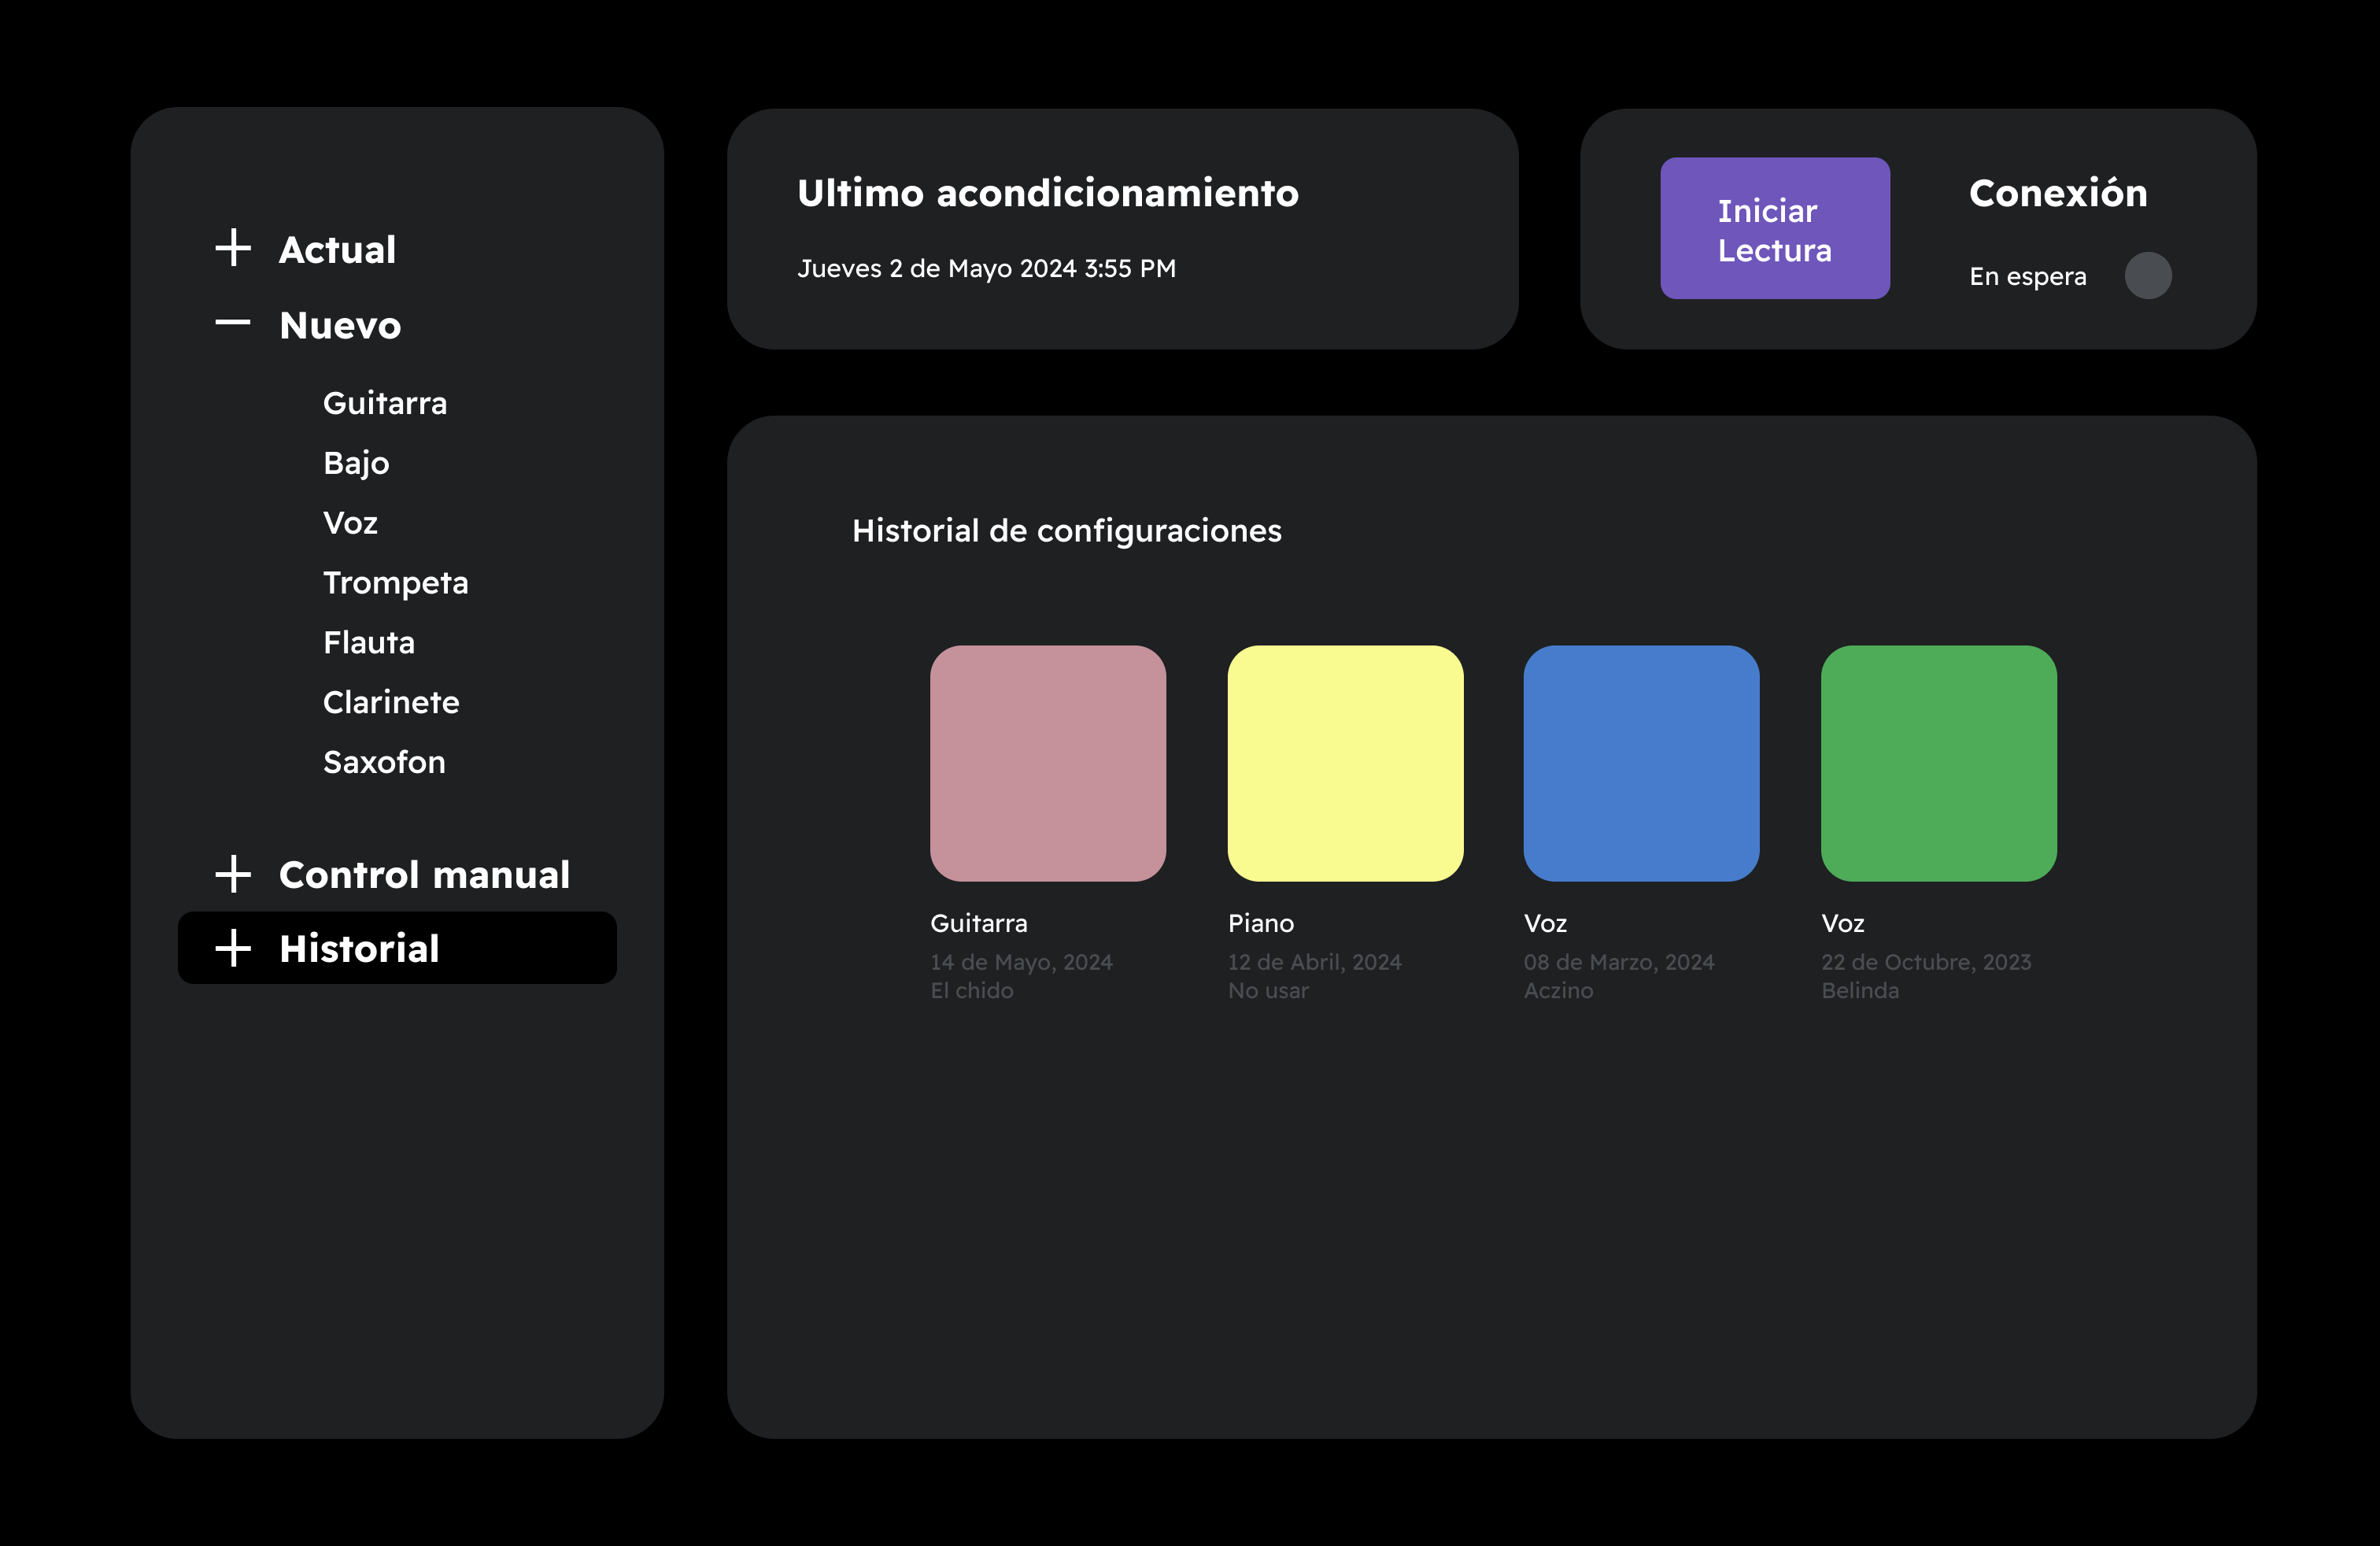
\includegraphics[width=\linewidth]{imagenes/Historial.png}
        \caption{\footnotesize Página del historial de configuraciones}
        \label{fig:pagina_historial}
    \end{subfigure}
    \caption{Vistas de la interfaz de usuario}
    \label{fig:vistas_interfaz}
\end{figure}
\FloatBarrier

Para el desarrollo ya de una manera técnica, hemos seleccionado tecnologías que nos permiten crear una aplicación robusta, eficiente y de fácil mantenimiento. La tecnología principal que utilizaremos es Electron, complementada con otras herramientas y marcos de trabajo. \\

\textbf{Electron}
\begin{itemize}[label={}, leftmargin=0pt]
    \item \textbf{Descripción:} Electron es un marco de trabajo para construir aplicaciones de escritorio utilizando tecnologías web HTML, CSS y JavaScript. Permite crear aplicaciones multiplataforma que pueden ejecutarse en Windows, macOS y Linux desde una única base de código.
    \item \textbf{Justificación:}
\end{itemize}

\begin{longtable}{|p{3cm}|p{10cm}|}
\hline
\textbf{Ventaja} & \textbf{Descripción} \\ \hline
Multiplataforma & Electron permite desarrollar una sola vez y desplegar en múltiples sistemas operativos, lo cual reduce el tiempo y los costos de desarrollo. \\ \hline
Tecnologías Web & Al utilizar HTML, CSS y JavaScript, podemos aprovechar la vasta cantidad de recursos, bibliotecas y herramientas disponibles en el ecosistema web. \\ \hline
Facilidad de Desarrollo & Electron simplifica la creación de interfaces de usuario atractivas y funcionales, lo que nos permite centrarnos en la lógica de negocio y la experiencia del usuario. \\ \hline
Comunidad y Soporte & Electron cuenta con una amplia comunidad de desarrolladores y una extensa documentación, facilitando la resolución de problemas y la implementación de características avanzadas. \\ \hline
\caption{Selección de marco de trabajo: Electron}
\end{longtable}

\textbf{React}
\begin{itemize}[label={}, leftmargin=0pt]
    \item \textbf{Descripción:} React es una biblioteca de JavaScript para construir interfaces de usuario. Permite crear componentes reutilizables que gestionan su propio estado, lo que facilita el desarrollo de aplicaciones dinámicas y responsivas.
    \item \textbf{Justificación:}
\end{itemize}

\begin{longtable}{|p{3cm}|p{10cm}|}
\hline
\textbf{Ventaja} & \textbf{Descripción} \\ \hline
Componentización & React permite dividir la interfaz de usuario en componentes reutilizables, lo que mejora la mantenibilidad y la escalabilidad del código. \\ \hline
Virtual DOM & React utiliza un DOM virtual para minimizar las actualizaciones en el DOM real, lo que mejora significativamente el rendimiento de la aplicación. \\ \hline
Comunidad y Ecosistema & React tiene una gran comunidad y un ecosistema robusto, con numerosas bibliotecas y herramientas que facilitan el desarrollo. \\ \hline
Aprendizaje y Uso & React es relativamente fácil de aprender y usar, con una sintaxis declarativa que simplifica la creación de interfaces de usuario complejas. \\ \hline
\caption{Selección de libreria de desarrollo principal: React}
\end{longtable}

\textbf{Redux}
\begin{itemize}[label={}, leftmargin=0pt]
    \item \textbf{Descripción:} Redux es una biblioteca de JavaScript para gestionar el estado de la aplicación de manera predecible. Comúnmente acompañada de React.
    \item \textbf{Justificación:}
\end{itemize}

\begin{longtable}{|p{3cm}|p{10cm}|}
\hline
\textbf{Ventaja} & \textbf{Descripción} \\ \hline
Manejabilidad del Estado & Redux proporciona una manera clara y predecible de gestionar el estado de la aplicación, facilitando la depuración y el mantenimiento del código. \\ \hline
Escalabilidad & Redux es adecuado para aplicaciones grandes y complejas donde el manejo del estado puede volverse complicado. \\ \hline
Ecosistema & Redux tiene un amplio ecosistema de herramientas y middleware que facilitan tareas comunes como la asincronía y la persistencia del estado. \\ \hline
\caption{Selección de gestor del estado: Redux}
\end{longtable}

\textbf{Styled Components}
\begin{itemize}[label={}, leftmargin=0pt]
    \item \textbf{Descripción:} Styled Components es una biblioteca de JavaScript que permite escribir estilos CSS dentro del código JavaScript utilizando una técnica llamada CSS-in-JS.
    \item \textbf{Justificación:}
\end{itemize}

\begin{longtable}{|p{3cm}|p{10cm}|}
\hline
\textbf{Ventaja} & \textbf{Descripción} \\ \hline
Encapsulación & Styled Components permite encapsular estilos dentro de los componentes, evitando conflictos de nombres y facilitando la mantenibilidad. \\ \hline
Dinamismo & Permite aplicar estilos dinámicos basados en props y estado, lo cual es ideal para interfaces de usuario interactivas. \\ \hline
Integración & Styled Components se integra perfectamente con React, permitiendo una experiencia de desarrollo fluida y consistente. \\ \hline
\caption{Selección de herramienta de estilizado: Styled Components}
\end{longtable}

\textbf{D3.js}
\begin{itemize}[label={}, leftmargin=0pt]
    \item \textbf{Descripción:} D3.js es una biblioteca de JavaScript para la visualización de datos que permite manipular documentos basados en datos.
    \item \textbf{Justificación:}
\end{itemize}

\begin{longtable}{|p{3cm}|p{10cm}|}
\hline
\textbf{Ventaja} & \textbf{Descripción} \\ \hline
Flexibilidad & D3.js permite crear visualizaciones de datos altamente personalizadas y interactivas. \\ \hline
Actualización Dinámica & Facilita la actualización dinámica de las visualizaciones en respuesta a cambios en los datos. \\ \hline
Comunidad y Recursos & D3.js cuenta con una amplia comunidad y una gran cantidad de recursos y ejemplos disponibles para aprender y resolver problemas. \\ \hline
\caption{Selección de herramienta de visualización: D3.js}
\end{longtable}

La combinación de Electron con React, Redux, Styled Components y D3.js funciona en sinergia de la siguiente manera: Electron para desarrollar la aplicación multiplataforma, React y Redux facilitan la construcción de la interfaz de usuario dinámica y gestionada de manera eficiente. Styled Components asegura que nuestros estilos sean modulares y mantenibles, y por ultimo D3.js nos permite ofrecer visualizaciones de datos ricas e interactivas.
Esta selección de tecnologías está cuidadosamente diseñada para satisfacer las necesidades de nuestro proyecto, garantizando tanto la experiencia de desarrollo, como el resultado para el usuario. \\
